\documentclass[11pt,slidestop,mathserif,compress]{beamer}
%\documentclass[handout]{beamer}
%[slidestop] puts frame titles & contents on the top left corner (default = [slidescentered])
%[red] changes navigation bars and title to reddish color
%[mathserif] use serif fonts for representing formulas instead of sans serif (default = mathsans)
%[notes] adds notes to PDF screen
%[compress] the navigationbar in one line
%[notesonly] make only notes

%\mode<presentation>
%\mode<article>

\usepackage{xeCJK}
%\usepackage{hyperref}
%\usepackage{amsmath} %for math AMS fonts
%\usepackage{graphicx} %to include figures
%\usepackage{subfigure} %to have figures in figures
%\usepackage{multimedia} %to include movies
\usepackage{amsfonts}
\usepackage{multicol}
\usepackage{graphicx}
\usepackage{array}

\usepackage{tikz}
\usetikzlibrary{shapes,arrows}
\usepackage[ruled]{algorithm2e}

\usepackage{collectbox}


%Fonts
\setCJKmainfont[BoldFont={Adobe Heiti Std}, ItalicFont={Adobe Kaiti Std}]{Adobe Song Std}
\setCJKsansfont{Adobe Kaiti Std}
\setCJKmonofont{Adobe Fangsong Std}
\setmainfont{Times New Roman}
\setsansfont{Candara}
\setmonofont{Bitstream Vera Sans Mono}


%NewCommands
\newcommand\abs[1]{\left\lvert #1 \right\rvert}
\newcommand\floor[1]{\left\lfloor #1 \right\rfloor}
\newcommand\ceil[1]{\left\lceil #1 \right\rceil}
\newcommand\yin[1]{\textit{#1}}
\newcommand\yang[1]{\textbf{#1}}


%Theme
%View on website: http://www.hartwork.org/beamer-theme-matrix/
\usetheme{Warsaw}
\usecolortheme{default}
%\useoutertheme[subsection=false]{smoothbars}
%\useinnertheme{rectangles}


%Style
\setbeamertemplate{footline}{}
%\setbeamertemplate{footline}{{\small\insertframenumber/\inserttotalframenumber}}
\setbeamertemplate{headline}
{%
	\leavevmode%
	\hbox{%
		\begin{beamercolorbox}[wd=.5\paperwidth,ht=2.65ex,dp=1.5ex,right]{section in head/foot}%
			\usebeamerfont{section in head/foot}\insertsectionhead\hspace*{2ex}
		\end{beamercolorbox}%
		\begin{beamercolorbox}[wd=.5\paperwidth,ht=2.65ex,dp=1.5ex,left,plus1fil,rightskip=.3cm]{subsection in head/foot}%
			\usebeamerfont{subsection in head/foot}\hspace*{2ex}\insertsubsectionhead\hfill\yang{\insertframenumber/\inserttotalframenumber}
		\end{beamercolorbox}}%
	\vskip0pt%
}
%\setbeamertemplate{theorem}[ams style]
%\setbeamertemplate{theorems}[numbered]
%\setbeamertemplate{lemmas}[numbered]

\makeatletter
\newenvironment<>{proofs}[1][\proofname]{%
    \par
    \def\insertproofname{#1\@addpunct{.}}%
    \usebeamertemplate{proof begin}#2}
  {\usebeamertemplate{proof end}}
\newenvironment<>{proofc}{%
  \setbeamertemplate{proof begin}{\begin{block}{}}
    \par
    \usebeamertemplate{proof begin}}
  {\usebeamertemplate{proof end}}
\newenvironment<>{proofe}{%
    \par
    \pushQED{\qed}
    \setbeamertemplate{proof begin}{\begin{block}{}}
    \usebeamertemplate{proof begin}}
  {\popQED\usebeamertemplate{proof end}}
\makeatother


%\useoutertheme{infolines}
%\beamertemplatetransparentcoveredhigh %makes all covered text highly transparent
%\beamertemplatetransparentcovereddynamicmedium %makes all covered text quite transparent, but is a dynamic way. The range of dynamics is smaller




%Animation
%\beamerdefaultoverlayspecification{<+->}
%Read Amber M. Smith




%PDF
%\hypersetup{pdfpagemode=FullScreen}


\begin{document}

%\input{fixbug.tex}

\title{Activity Recognition using integrated sensors}
\author{{\bfseries 李健} \\ {\bfseries 101220055} \\ {\scriptsize <lijianxp2005@gmail.com>}}
\institute{Nanjing University}
\subject{Computer Science}
\date{June, 2013}

%\title[Crisis] % (optional, only for long titles)
%{The Economics of Financial Crisis}
%\subtitle{Evidence from India}
%\author[Author, Anders] % (optional, for multiple authors)
%{F.~Author\inst{1} \and S.~Anders\inst{2}}
%\institute[Universitäten Hier und Dort] % (optional)
%{
%	\inst{1}%
%	Institut für Informatik\\
%	Universität Hier
%	\and
%	\inst{2}%
%	Institut für theoretische Philosophie\\
%	Universität Dort
%}
%\date[KPT 2004] % (optional)
%{Konferenz über Präsentationstechniken, 2004}
%\subject{Informatik}

%[plain] for plane frame style
%[containsverbatim] for using verbatim environment and \verb command
%[allowframebreaks] for automatic split of frames if the contents do not fit in a single slide
%[shrink] for shrinking the contents to fit in a single slide
%[squeeze] for squeezing vertical space

\begin{frame}[plain]
	\titlepage
\end{frame}

%\begin{frame}[shrink]
%	\frametitle{Contents}
%	\begin{multicols}{2}
%		\tableofcontents
%	\end{multicols}
%\end{frame}

\section{Idea}

\begin{frame}
	\transdissolve<1>
	\frametitle{Big Picture}
	\tikzstyle{A} = [draw, thin, fill=blue!20]
	\tikzstyle{B} = [ellipse, draw, thin, fill=green!20, minimum height=2.5em]

	\resizebox{1\textwidth}{!}{
		\begin{tikzpicture}[node distance = 3.8cm, auto, >=latex', thick]
			\node [A] (compress) {Compression};
			\node [B, below of=compress] (data) {Sensors Data};
			\node [A, right of=compress] (fe) {Feature Extration};
			\node [A, right of=fe] (classification) {Classification};
			\node [A, right of=classification,node distance = 4.2cm] (model) {Model};
			\node [B, below of=model] (result) {Result};
			\node [A, left of=result] (arbiter) {Arbiter};
			\node [B, left of=arbiter] (label) {Label};
			\node [A, node distance = 1.9cm, below of=compress] (split) {Split};

			\path[->] (compress) edge (fe);
			\path[->, dashed] (fe) edge (classification);
			\path[->, dashed] (classification) edge node[auto,midway] {Training} (model);
			\path[->] (model) edge (result);
			\path[->] (fe) edge [bend left] (model);
			\path[->] (model) edge node[auto,midway] {Prediction} (result);
			\path[->,dashed] (result) edge node[auto,midway,above] {Recovery} (arbiter);
			\path[->,dashed] (result) edge [bend left] (arbiter);
			\path[->,dashed] (result) edge [bend right] (arbiter);
			\path[->] (arbiter) edge (label);
			\path[->] (data) edge (split);
			\path[->,dashed] (split) edge (compress);
			\path[->,dashed] (split) edge [bend left] (compress);
			\path[->,dashed] (split) edge [bend right] (compress);
		\end{tikzpicture}
	}
\end{frame}

\section{Method}

\subsection{Observation}
\begin{frame}
	\frametitle{Observation}
	\begin{figure}[H]
		\centering
		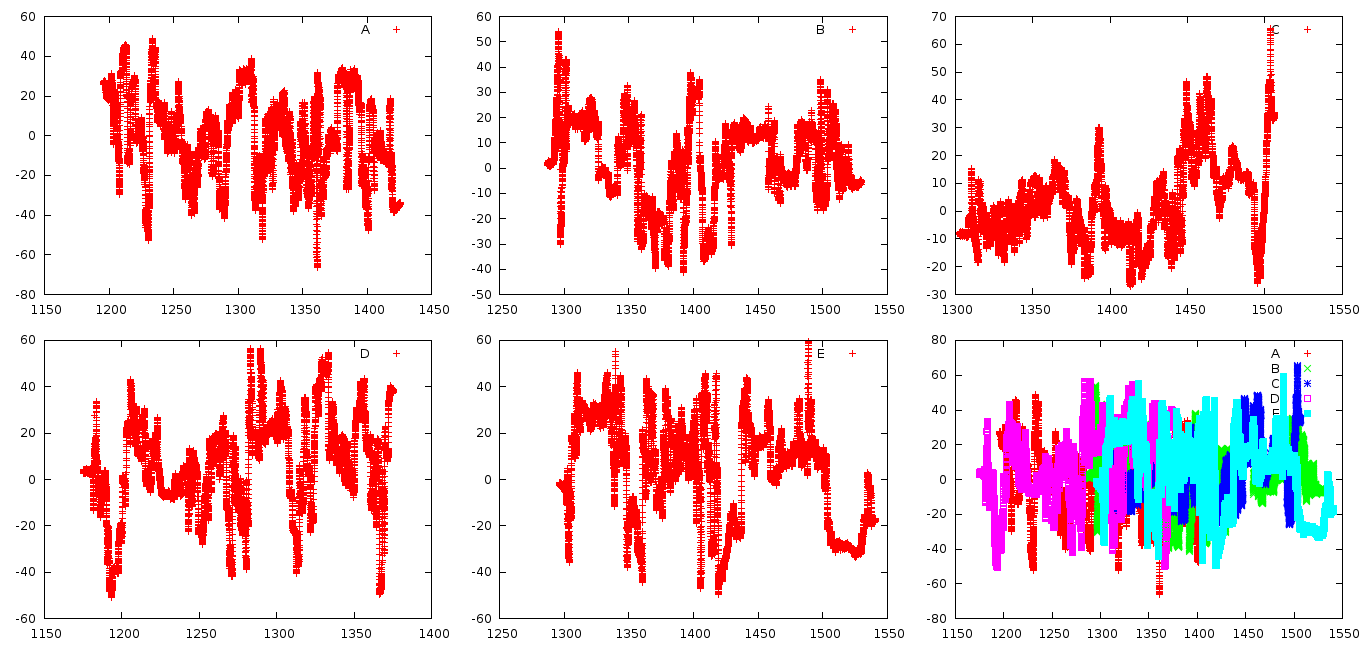
\includegraphics[width=1.0\textwidth]{B.png}
		\caption{Discrete time-series data of the same activity in different data set}
	\end{figure}
\end{frame}

\subsection{Preprocessing}
\begin{frame}
	\frametitle{Split}
	\begin{block}{Procedure}
		\begin{itemize}
			\item	Splitting raw data by Label
			\item	Remapping Label to $\{-1, 1\}$
		\end{itemize}
	\end{block}
	\pause
	\begin{exampleblock}{Multi-Class Classification $\Rightarrow$ Two-Class Classification}
		\begin{itemize}
			\item	Using different model
			\item	More accuracy
		\end{itemize}
	\end{exampleblock}
\end{frame}

\begin{frame}
	\frametitle{Compress}
	\begin{block}{Procedure}
		\begin{itemize}
			\item	Combine every $\alpha$ raw data
			\item	Average
		\end{itemize}
	\end{block}
	\pause
	\begin{exampleblock}{Smooth}
		\begin{itemize}
			\item	Eliminate unknown data
			\item	Smooth extreme data
			\item	Reduce scale of raw data
		\end{itemize}
	\end{exampleblock}
\end{frame}

\subsection{Data Transform and Extract Features}

\begin{frame}
	\frametitle{Observation}
	\begin{figure}[H]
		\centering
		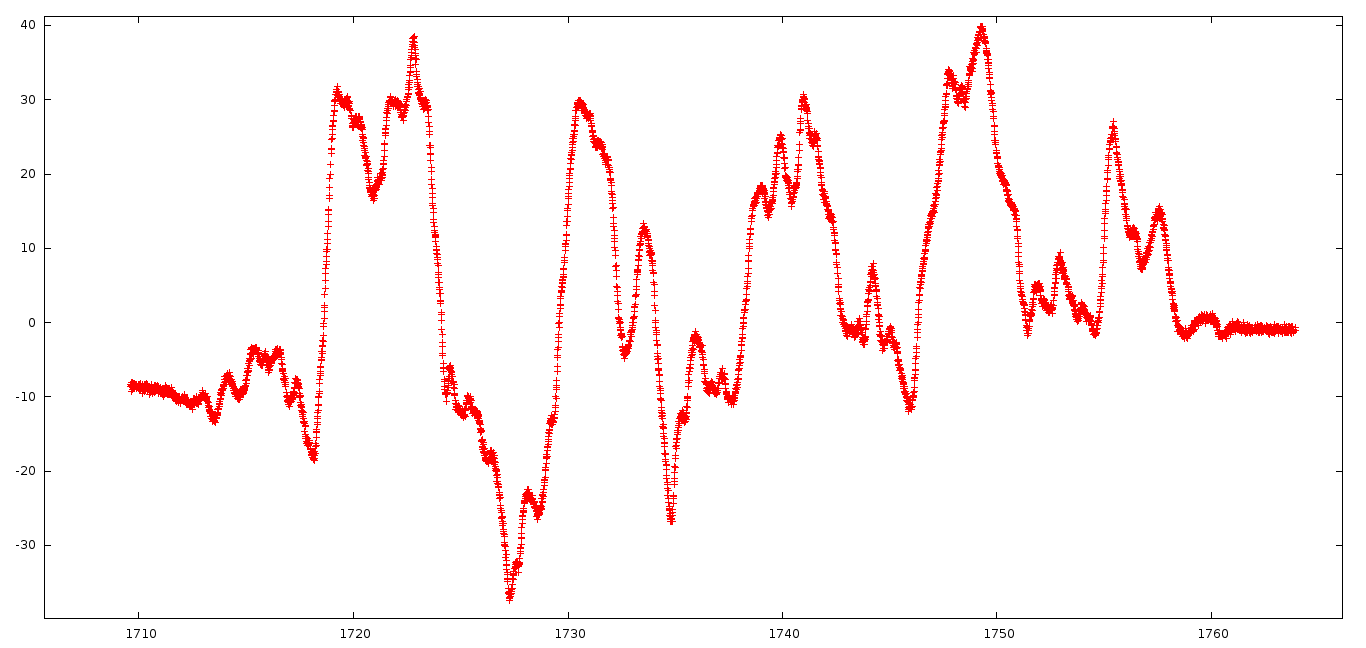
\includegraphics[width=1.0\textwidth]{A.png}
		\caption{Discrete time-series data}
	\end{figure}
\end{frame}

\begin{frame}
	\frametitle{Time-Series}
	\begin{block}{Continous vs. Discrete}
		Every $\beta$ time-based data point $\Rightarrow$ Features
	\end{block}
	\begin{exampleblock}{Features}
		\begin{itemize}
			\item	Average: $\bar{X}$
			\item	Variance: $\frac{1}{n} \sum (X_i - \bar{X})^2$
			\item	$\max{X_i} - \min{X_i}$
			\item	$X_1 - X_n$
			\item	$\frac{1}{n}\sum \abs{X_i - \bar{X}}$
			\item	Time between Peaks
			\item	Binned Distribution
			\item	Discrete Wavelet Transform: Haar
		\end{itemize}
	\end{exampleblock}
\end{frame}

\begin{frame}
	\frametitle{Time between Peaks}
	\begin{figure}[H]
		\centering
		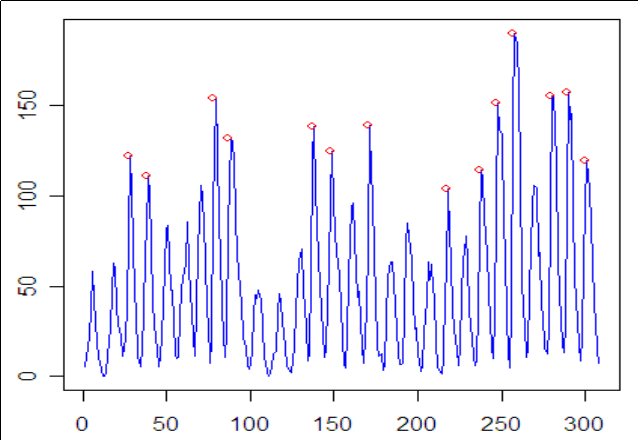
\includegraphics[width=0.8\textwidth]{C.png}
		\caption{Peaks Detection}
	\end{figure}
\end{frame}

\begin{frame}[shrink]
	\frametitle{Time between Peaks}
	\begin{exampleblock}{Algorithm}
		\begin{algorithm}[H]
			\caption{Peak Detection Algorithm that uses Peak Function F}
			\DontPrintSemicolon
			\SetKwInOut{Input}{Input}
			\SetKwInOut{Output}{Output}
			\SetKw{And}{and}
			\Input{Time-series of $N$ points: $X = \{x_1, x_2, \cdots, x_N\}$, $N$ \\  Window size around the peak: $K$ \\ Threshold: $H$}
			\Output{Set of peaks detected in $X$: $S$}
			\BlankLine
			\Begin{
				$S = \emptyset$\;
				\For{$i = 1$ \KwTo $N$}
				{
					$A[i] = F(X, i, K)$\;
				}
				Compute the mean $avg$ and standard deviati n $var$ of all values in array $A$\;
				\For{$i = 1$ \KwTo $N$}
				{
					\If{$A[i] > 0$ \And $(A[i] - avg) > H \cdot var$}
					{
						$S = S \cup \{x_i\}$\;
					}
				}
				\For{every adjacent pair of peaks $x_i$ and $x_j$ in $S$}
				{
					\If{$|j - i| \leq K$}
					{
						Remove the smaller value of $\{x_i, x_j\}$ from $S$\;
					}
				}

			}
		\end{algorithm}
	\end{exampleblock}
\end{frame}

\begin{frame}
	\frametitle{Binned Distribution}
	\begin{figure}[H]
		\centering
		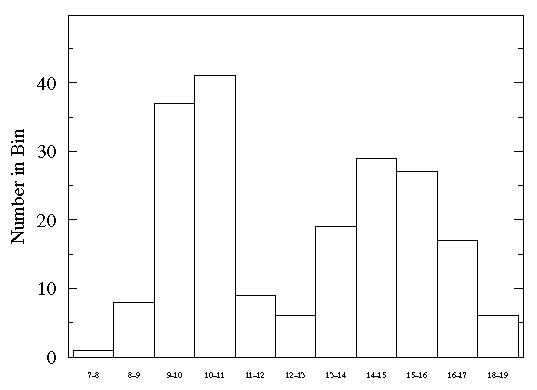
\includegraphics[width=0.8\textwidth]{D.png}
		\caption{Binned Distribution}
	\end{figure}
\end{frame}

\begin{frame}
	\frametitle{Discrete Wavelet Transform: Haar}
	\begin{block}{Procedure}
		\begin{itemize}
			\item	1D Haar Wavelet Transform
			\item	Largest 5 components
		\end{itemize}
	\end{block}
	
	\pause
	\begin{exampleblock}{Period}
		Describe the period of the time-series data
	\end{exampleblock}

\end{frame}

\subsection{Training and Predicting}

\begin{frame}
	\frametitle{Training and Predicting}
	\begin{block}{Support Vector Machine}
		\begin{itemize}
			\item	RBF Kernel
			\item	Two-Class Classification
			\item	Performance
		\end{itemize}
	\end{block}
	\pause
	\begin{block}{Recovery}
		\begin{itemize}
			\item	Expand
		\end{itemize}
	\end{block}
\end{frame}

\subsection{Arbiter}
\begin{frame}
	\frametitle{Arbiter}
	\begin{block}{Procedure}
		\begin{itemize}
			\item	Collect the vote from all models
			\item	For each data
					\begin{itemize}
						\item	$1$ Positive $\Rightarrow$ Confirmed
						\item	$0$ Positive $\Rightarrow$ Unknown
						\item	$>1$ Positive $\Rightarrow$ Confused
					\end{itemize}
			\item	If "Confused" $\Rightarrow$ $Score_i = F(Model_i, Probability_i, Estimate_i)$
		\end{itemize}
	\end{block}
\end{frame}

\section{Result}
\begin{frame}[shrink]
	\transdissolve<1>
	\frametitle{Result}
	\begin{block}{Parameters}
		\begin{table}[h]
			\centering
			\resizebox{1\textwidth}{!}{
				\begin{tabular}{cccccccc}
					\hline
					Activity & $\alpha$ & $\beta$ & Training Data & Temperature & Haar & Time between Peaks & Binned Distribution\tabularnewline
					\hline
					 1 & 40 & 20 & ABCDE & + & - & + & +\tabularnewline
			2 & 50 & 20 & DE & - & + & - & -\tabularnewline
		 3 & 10 & 100 & BCDE & - & + & - & -\tabularnewline
		 4 & 50 & 20 & ABCDE & - & - & - & +\tabularnewline
		 5 & 50 & 50 & BDE & - & - & + & +\tabularnewline
		 6 & 50 & 20 & ABCDE & - & - & - & +\tabularnewline
		 7 & 50 & 20 & ABCDE & - & - & - & +\tabularnewline
		12 & 50 & 20 & ABDE & + & + & - & -\tabularnewline
		13 & 50 & 50 & BDE & - & - & - & +($|Bins|=5$)\tabularnewline
		16 & 50 & 20 & ABCDE & + & + & - & -\tabularnewline
		17 & 50 & 50 & ABCDE & - & + & - & -\tabularnewline
		24 & 50 & 20 & ABCDE & + & - & + & +\tabularnewline
					\hline
				\end{tabular}
			}
		\end{table}
	\end{block}
	\begin{exampleblock}{Result}
		\begin{table}[h]
			\centering
			\resizebox{1\textwidth}{!}{
				\begin{tabular}{cccccccccccccccc}
					\hline
					Activity & 1 & 2 & 3 & 4 & 5 & 6 & 7 & 12 & 13 & 16 & 17 & 24 & Sum & Best & Worst\tabularnewline
					\hline
					$F_1$ & 0.9938 & 0.9884 & 0.9763 & 0.9451 & 0.9872 & 0.9372 & 0.9690 & 0.8577 & 0.8681 & 0.8819 & 0.9718 & N/A & 10.3766 & 0.9938 & 0.8577\tabularnewline
					\hline
				\end{tabular}
			}
		\end{table}


	\end{exampleblock}
\end{frame}

\begin{frame}
	\transdissolve<1>
	\frametitle{Thank you!}
\end{frame}

\end{document}

